\section{Dise�o}
\label{21:sec:Disenyo}

\subsection{Componentes del sistema}
\label{s2:subsec:sistema-entero}
A la hora de realizar el sistema, se ha decidido utilizar los siguientes
componentes:
\begin{itemize}
\item \emph{FGPA}, que como se ha comentado en la secci�n anterior, es la
  encargada de realizar los c�lculos del juego, interpretar las �rdenes de
  los usuarios, y mostrar el juego mediante un monitor VGA.
\item \emph{Maletines ARM}, encargados de leer las �rdenes de los
  jugadores (mediante pulsaciones en el teclado matricial o los botones de
  la placa) y transmitirlas a la FPGA mediante una UART. Como la FPGA
  utilizada �nicamente posee una UART, los maletines se pueden conectar en
  serie, y transmitir los mensajes de uno hacia el siguiente hasta que
  lleguen a la FPGA (ver secci�n~\ref{s3:subsec:maletines}). Adem�s, la
  FPGA transmite la informaci�n de puntuaci�n a los maletines, los cuales
  la muestran mediante sus \emph{Display 8-Segmentos}.
\item \emph{Display 8-Segmentos}, utilizado para mostrar la informaci�n de
  puntuaci�n.
\item \emph{Pulsadores y teclado matricial}, para que los jugadores
  indiquen sus �rdenes de movimiento al sistema.
\item \emph{Monitor VGA}, utilizado para mostrar el juego.
\end{itemize}

En la subsecci�n~\ref{s2:subsec:comportamiento} se muestra el
comportamiento del sistema, mientras que en la
subsecci�n~\ref{s2:subsec:comunicacion} el diagrama de comunicaci�n entre
los componentes aqu� descritos.
\subsection{Comportamiento del sistema}
\label{s2:subsec:comportamiento}
Aqu� habr�a que poner diagramas de comunicaci�n, secuencia, m�quina de
estados, los que consideremos oportunos.


\subsection{Comunicaci�n entre componentes}
\label{s2:subsec:comunicacion}
\begin{figure}[h]
  \centering
  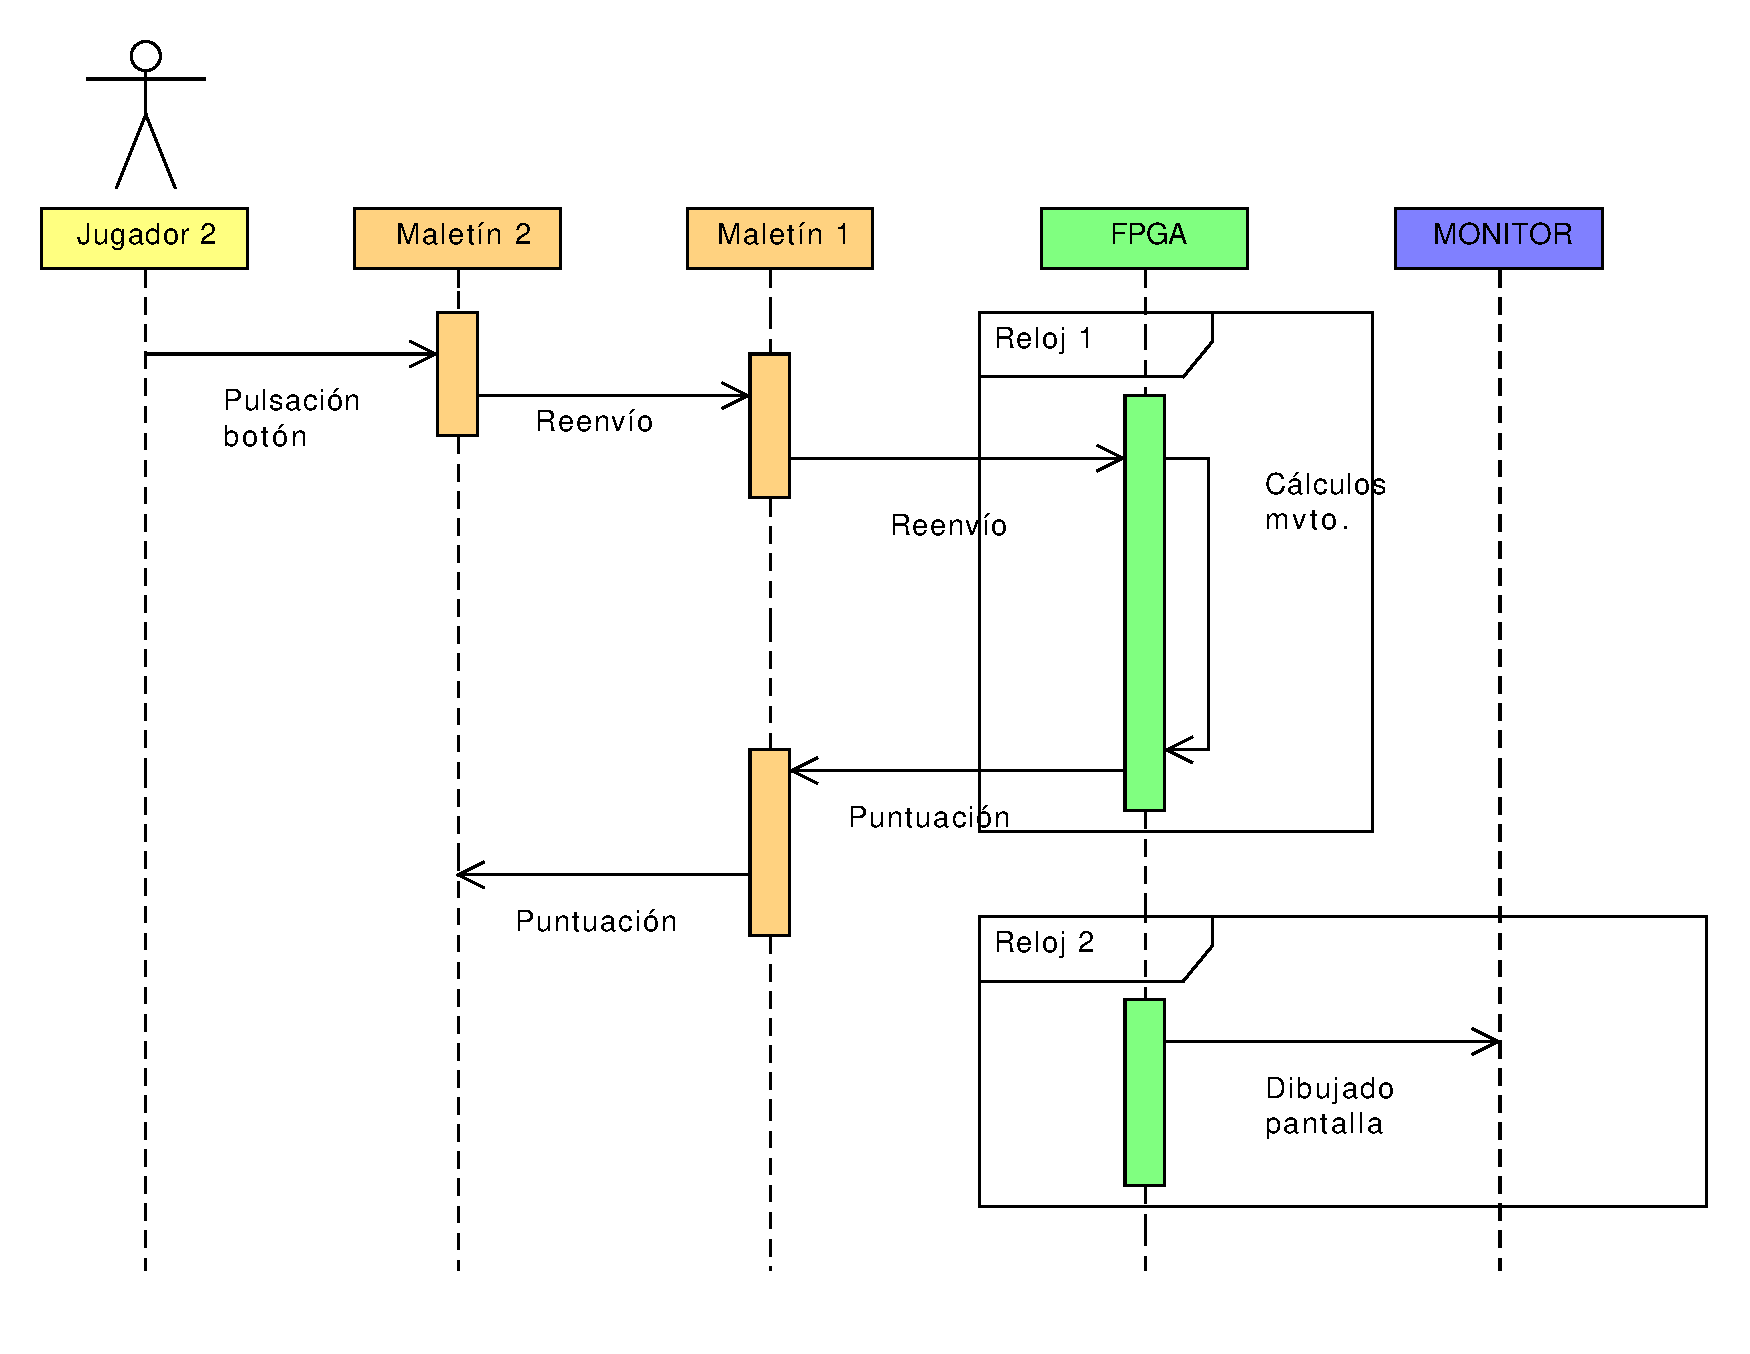
\includegraphics[width=1.0\textwidth]{images/secuencia.pdf}
  \caption{Diagrama de secuencia entre los distintos componentes.}
  \label{s2:fig:secuencia}
\end{figure}


%
%
%%%
%%% Local Variables:
%%% mode: latex
%%% TeX-master: "../main.tex"
%%% End:


